In this work we have investigated behaviour of task-affinity on different architectures. Task-affinity is based on assumption that, if tasks share a great 
amount of data and we have an SMP architecture, then occasionally executing them on the first available processors will increase the cache-miss rate. If we 
move tasks to be executed near to where data was produced, then we spare some cache-misses \cite{lcs}. We have demonstrate that this assumption is not 
always true. Migrations of tasks play an important role on predictability of the applications. When a task migrates, data could be moved from one cache to 
another. As we have seen on Intel Xeon and as it is demonstrated in \cite{molka}, this operation may involve high latency that depends on cache 
architecture, inter-chip communications and other hardware factors. Therefore it is clear that it is not enough to execute tasks that share common data 
on the same CPUs, but it is necessary guarantee that tasks that share common data find what they need possibly in L1 cache. For this reason, we have 
improved the concept of temporal locality.

The experimental results show that task-affinity is effective on Intel i7, where there is an average speedup in term of A2S of $\sim 17\%$. We have 
increased task migration, nevertheless we have improved throughput and predictability. It is clear that architecture of Intel i7 mitigates the side effects 
of the high number of migrations of tasks. On Intel Xeon task-affinity is effective only with buffer greater than 4KB, in that case there is an average 
speedup in term of A2S of $\sim 10,5\%$. It is clear that the effect of migrations of tasks is more significant on this architecture.

We could obtain results still better with a more effective migration policy. In this patch, in order to improve the temporal locality, we have included 
\textit{push\_rt\_task} in the task-affinity logic and we have seen that, because of the scheduling performed, \textit{pull\_rt\_task} has an higer overhead
than vanilla. 

We conclude that the mechanism proposed brought, in fact, an improvement of throughput and on determinism of the entire application, especially with buffers
of big dimension as 32KB. It is interesting that these improvements take place even if L1 and LLC miss rates increase (Intel Xeon) therefore it is clear
that, according to the cache architecture used, cache misses have a different impact on performance of application.


%%%%%%%%%%%%%%%%%%%%%%%%%%%%%%%%%%%%%%%%%%%%%%%%%%%%%%%%%%%%%%%%%%%%%%%
\section{Future Works}

During the development of task-affinity, NUMA architectures were never considered. In the final part of this thesis we have started to analyze the 
behaviour of task-affinity on AMD Opteron, a NUMA architecture. In a first trial, using some kernel facilities, we have held all tasks to be executed only 
on one node, in order to simulate an SMP architecture. We have obtained the following results:

\begin{figure}[htbp]
\centering
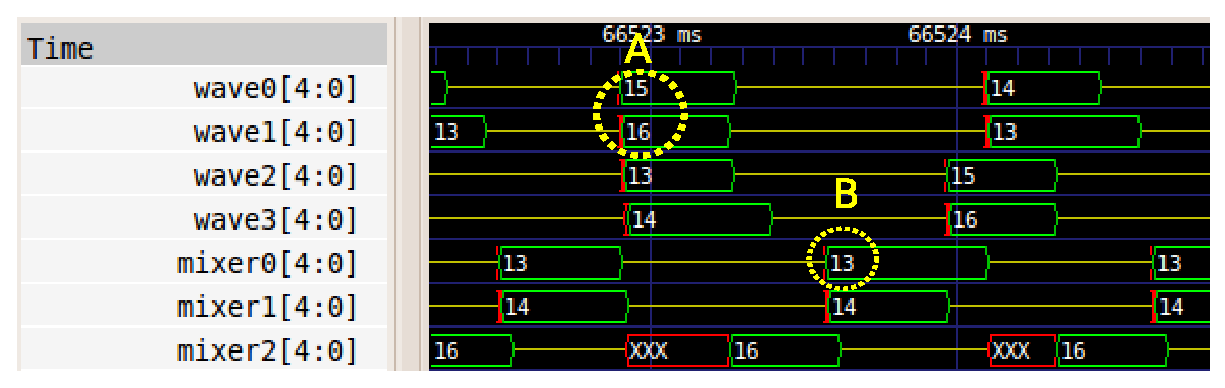
\includegraphics[width=\widefigure]{images/results_AMD/final_AMD.eps}
\caption{\figurecaption{Scheduling performed by new version of task-affinity on Opteron (new version of task-affinity)}}
\label{fig:trace_AMD}
\end{figure}

\begin{figure}[htbp]
\centering
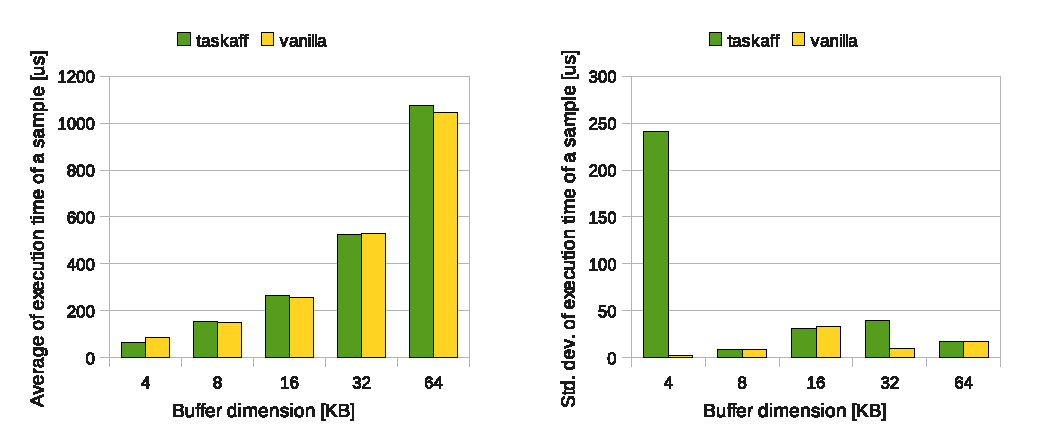
\includegraphics[width=\widefigure]{images/results_AMD/time_avg_var_AMD.eps}
\caption{\figurecaption{Average and Variance of execution time of a sample Opteron (new version of task-affinity)}}
\label{fig:time_avg_var_AMD}
\end{figure}

Task-affinity on this machine doesn't work properly. We can see in step B that \textit{mixer0} doesn't choose the correct CPU. The incorrect behaviour of 
task-affinity is also reflected by Fig. \ref{fig:time_avg_var_AMD}, where we can see a worsening of throughput and predictability. It is possible that the 
task-affinity doesn't work, because of a lot of kernel threads used to manage load balancing and others kernel activities in NUMA architectures: but this is 
only an hypothesis. According these results, it is clear that task-affinity needs the support for NUMA architectures, this is the first step to improve 
task-affinity.

In this work, we have seen that cache misses have a different impact on determinism of application on different architectures, it is necessary to 
estimate how much cache misses impact on application performance and in particular on determinism, in order to understand if the task-affinity could 
improve significantly or not the determinism of application on a given architecture. 

Another possible improvement is to optimize the migration policy, in order to include also \textit{pull\_rt\_task} in task-affinity logic and finally, it 
would be better not to use system calls to define dependencies among tasks, but, instead, to rely in other mechanisms, such as a profiler \cite{calandro}, 
that infers automatically the dependencies among tasks. The reason is that it is not desirable to modify present applications to use the task-affinity. 
The mechanism of adding and removing dependencies would be rather the same: only the user interface would need to be changed.

